\documentclass{article}

\usepackage{geometry}
\geometry{margin=2cm}
\usepackage{graphicx}
\usepackage{hyperref}
\usepackage{amsfonts}
\usepackage{caption}
\usepackage{subcaption}

\hypersetup{colorlinks=true, linkcolor=blue, urlcolor=blue}
\urlstyle{same}
\begin{document}
	
	\author{Aayush Arya}
	\date{(Submitted: November 1, 2021)}
	\title{}
	
	\maketitle
	
	\hrule
	\begin{center}
		PHY366 Lab Report\\
		Practical: 7 \quad Registration No.: 11912610 \quad Section: G2903
	\end{center}
	\hrule
	
	\section*{Aim}
	To study the input/output characterisitics and frequency response of a Common Emitter (CE) amplifier.
	
	\section*{Methods}
	
	We simulated a transistor circuit biased in the common emitter configuration and first characterized the input and output characteristics of the transistor.
	
	\begin{figure}[!h]
		\centering
		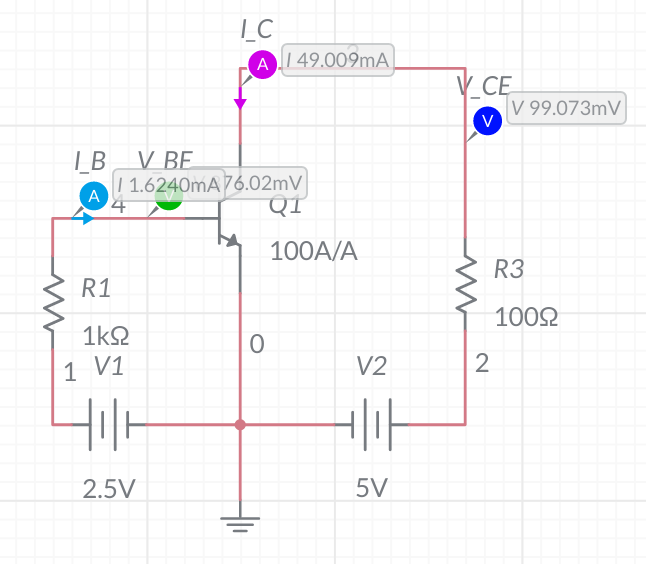
\includegraphics[width=0.6\textwidth]{io_chars}
	\end{figure}
	
	The circuit for input/output characterisation can be found at
	
	 \url{https://www.multisim.com/content/pEMRiTJNNADTw8LLDJV9pF/common-emitter-transistor-characteristics/open/}.
	 
	 
	\section*{Results \& Conclusions}
	We summarize the I/O characteristics below.
	\pagebreak
	\begin{figure}[!h]
		\centering
		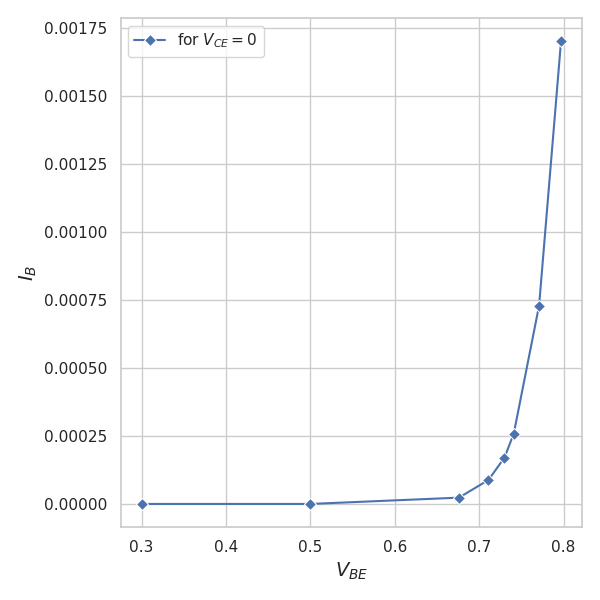
\includegraphics[width=0.5\textwidth]{input_chars}
		\caption{Input characteristics of a CE transistor for $V_{CE}=0$.}
		\label{fig:in}
	\end{figure}

	As expected, the input characteristics show the behavior of a pn-junction diode, with an exponentially increasing $I_B$ with $V_{BE}$. This is illustrated in Figure \ref{fig:in}.

	\begin{table}[!h]
		\centering
		\begin{tabular}{|c|c|}
			\hline
			$V_{CE}$ (Volts) & $I_C$  (mA) \\
			\hline
			0        & -0.166.04\\
			1        & 9.45    \\
			2        & 19.29   \\
			3        & 29.177  \\
			5        & 49.0    \\
			10       & 98.68   \\
			12       & 118.53  \\
			13       & 128.44  \\
			15       & 148.14  \\
			20       & 159.46  \\
			100      & 159.46 \\
			\hline
		\end{tabular}
		\caption{Observations of the output characteristics taken at $I_B = 1.6$ mA.}
	\end{table}
	
	We enumerate the measurements of the output characteristics in Table 1. Clearly, the output voltage saturates at $V_{CE} = 20$ V. This is shown in Figure \ref{fig:out}.

	\begin{figure}[!h]
		\centering
		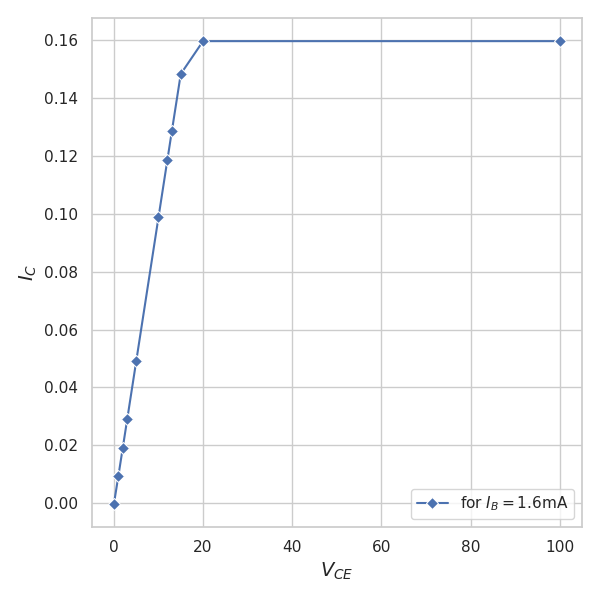
\includegraphics[width=0.5\textwidth]{output_chars}
		\caption{Output characteristics for the described CE configuration, at constant base current $I_B = 1.6$ mA.}
		\label{fig:out}
	\end{figure}
	
\end{document}